\documentclass[output=paper,modfonts,nonflat,newtxmath]{langsci/langscibook}
\author{Carmen Muñoz\affiliation{Universitat de Barcelona}}
\title{Cognate recognition by young multilingual language learners: The role of age and exposure}

\abstract{The present study set out to investigate the recognition of cognates by young multilingual  learners of English as a foreign language. While there is a wealth of research on the role of cognates in vocabulary recognition by bilingual children, much less is known in relation to bilinguals learning a foreign language with limited exposure to that language. The specific research questions that guided the study were i) To what extent do young Spanish-Catalan bilingual learners of English recognise English cognate words over non-cognate words in the PPVT test? and ii) What are the respective roles of age (7 vs. 9 years) and amount of exposure to English in cognate word recognition and non-cognate word recognition? Do these factors have the same roles in non-cognate word recognition? To answer these questions, the study examined the extent to which young learners recognised cognates in the Peabody Picture Vocabulary Test (PPVT) (\citealt{DunnDunn2007}). Participants were 170 children distributed into a group of 7 year-olds and a group of 9 year-olds. They were all Spanish-Catalan bilinguals, so that English was their third language. The results of the analyses indicated that age was the strongest determinant of cognate word recognition, whereas hours of exposure was the stronger predictor of non-cognate word recognition.}
% \keywords{{{cognates,} {multilingual} {learners,} {young} {learners,} {exposure,} {PPVT}}}

\shorttitlerunninghead{Cognate recognition by young multilingual language learners}
\begin{document}
\maketitle

\section{Introduction}

An important issue in studies in second language (L2) learning is whether learners can use their first language (L1) vocabulary knowledge to identify, interpret, and use target language vocabulary (\citealt{MendezPerezEtAl2010}). Cognates are defined as word pairs in two different languages that share both meaning (translation equivalents) and form (phonological or orthographic similarity) \citep{KohnertEtAl2004}. This definition subsumes three types of cognates: words that are phonologically similar and orthographically identical, words that are phonologically similar but orthographically different, and false cognates in which words are phonologically and orthographically similar but not related in meaning (e.g., Spanish \textit{embarazada} and English \textit{embarrassed}) (e.g., \citealt{Rodriguez2001}).

Cognates have been extensively studied in language processing and learning in bilinguals, but their role in foreign language learning has been somehow neglected in research in spite of the fact that it has always been commonly acknowledged that closely related languages are easier and faster to learn. In fact, one manifestation of cross-linguistic influence or transfer is that learning a new language will be facilitated by the resemblance of that language with a language or languages known to the learner, in particular in receptive tasks \citep{Ringbom2007}. This is the case of cognate words, which will be more likely noticed by the learner in the input and thus also more likely processed and retained in long-term memory. Certainly, research on L2 vocabulary learning has shown that the lexico-semantic representations of new words are better established when they overlap with the native language at form-based linguistic levels (orthography and phonology). In other words, cognates are easier to learn and integrate into the lexicon (e.g., \citealt{EllisNBeaton1993}; \citealt{DeGrootvanHell2005}).

One of the reasons for the relative neglect of cognates in foreign language learning research in the last decades has been the emphasis on the use of the target language in the classroom downplaying the role of the learners’ native language, although this is currently changing thanks to the influence of teaching perspectives favouring translanguaging in the classroom, which entails using one language to reinforce the other (e.g., \citealt{Williams2002}; \citealt{GarcíaLin2016}). In addition, communicative language teaching has been somehow perceived as in opposition to explicit approaches to teaching, precluding the teacher’s promotion of learners’ metalinguistic awareness. This has been especially the case in the young learners’ classroom. However, although there are few pedagogically oriented studies on the use of cognates (see \citealt{Otwinowska2016}), there is now some evidence that instruction designed to raise cross-linguistic awareness of cognates helps school learners recognise similarities between words that were previously unnoticed (\citealt{WhiteHorst2012}), which can boost learners’ vocabulary and general L2 proficiency. The main aim of the current study is to shed more light on children’s ability to recognise cognates by examining young foreign language learners’ recognition of cognates and the role of age and exposure to (or contact with)\footnote{Although the term “contact” may be more adequate than “exposure” in that it also implies productive use of the language, both terms are used indistinctly in this paper.} the foreign language. In addition, the study gathers evidence from bilingual (Spanish-Catalan) learners of a third language (English), which will be especially valuable for future studies addressing differences in cognate recognition in different multilingual constellations.

\section{Literature review}


\subsection{Cognate processing: the cognate facilitation effect}

The cognate facilitation effect refers to the well-documented finding in bilingual studies that cognate words are easier and faster to recognise than non-cognate words (e.g., \citealt{CaramazzaBrones1979}; \citealt{CostaEtAl2000}). There is a wealth of research on cognate processing (e.g., \citealt{VanHellDeGroot1998}; \citealt{DijkstraEtAl1999}), with important implications for theories of the bilingual mental lexicon/models of lexical access. A well-established finding from studies on lexical access is that word recognition in a second (or foreign) language is influenced by the native language (e.g., \citealt{KrollDijkstra2002}) and that the degree of reliance on the native language depends upon L2 proficiency.

 {Research has pointed out that the cognate facilitation effect decreases as a function of proficiency, possibly suggesting lower reliance on native language representations at higher proficiency levels \citep{KrollEtAl2010}. Confirmation of this relationship was also found in a study with adult foreign language learners by \citet{CasaponsaEtAl2015} in which they explored the strength of the cognate effect as a predictor factor of reading comprehension in two groups of English as a foreign language (EFL) learners at different levels of proficiency. The cognate effect was measured by subtracting reaction times to cognate words from reaction times to non-cognate words in a lexical decision task. The cognate effect was found to be a significant predictor of reading comprehension scores for both groups, but the relationship was positive for the lower proficiency group (level A2 of the CEFR), whereas the degree of reliance on cross-linguistic similarity appeared inversely related to reading comprehension achievement in learners at the relatively higher level of proficiency (level B1). According to Casaponsa and colleagues, this finding suggests a decrease on the strength of L1 reliance in favour of the direct links between L2 lexical representations and semantic concepts, in line with the predictions of current theoretical models (e.g., \citealt{KrollStewart1994}).}

 {Only a limited amount of research has addressed cognate processing in trilinguals (\citealt{VanHellDijkstra2002}; \citealt{LemhoferEtAl2004}; \citealt{Szubko-Sitarek2011}; \citealt{PoarchvanHell2012}). A pioneer study was conducted by \citet{VanHellDijkstra2002} with two groups of trilingual young adults, with Dutch as their native language and English and French as foreign languages. In one group, participants’ proficiency in English (L2) was higher than in French (L3), and in the other group their proficiency levels in L2 and L3 were comparable. The aim of the study was to examine whether knowledge of a weaker language would influence performance on words in the dominant language (L1). Participants were presented with word stimuli in their L1; one set of words were cognates with English, one set were cognates with French, and one set consisted of non-cognates. The study found that word association and lexical decision times in the two groups of trilinguals were shorter for words that were cognates with their L2 translations than for words that were non-cognates. For words that were cognates with their L3 translations, a cognate effect was only found in the group with high proficiency in that language.}

{In other words, a cognate advantage was noticeable only when the speaker was relatively proficient in the non-native language. Similar results were obtained in a study with young children including L2 learners, bilinguals and trilinguals by \citet{PoarchvanHell2012}. Results indicated a bidirectional cognate facilitation effect but only for bilinguals and trilinguals. For L2 learners only an effect from L1 to L2 was found, which led Poarch \& van Hell to conclude that lower levels of proficiency in an additional language allows only limited cross-linguistic activation.}


\subsection{Children’s recognition of cognates}

Research that focuses on the spontaneous recognition of cognates by children who have not been instructed to recognise them is especially interesting for the present study. Most research about these children’s ability to use cognates as a vocabulary learning strategy or their ability to recognise cognates indicates that, like adults, bilingual and trilingual children also show a cognate facilitation effect (\citealt{PoarchvanHell2012}; \citealt{PotapovaEtAl2016}).

Most studies with bilingual children in the US have employed the Peabody Picture Vocabulary Test (PPVT; \citealt{DunnDunn1981, DunnDunn1997}), a standardised receptive vocabulary test, to investigate the potential for a cognate advantage. \citet{UmbelEtAl1992} evaluated first graders’ performance on the PPVT and the Spanish version, Test de Vocabulario en Imágenes Peabody (TVIP; \citealt{DunnEtAl1986}). Children from Spanish monolingual and Spanish-English bilingual homes in US achieved similar overall scores on both tests and children responded correctly to cognates and non-cognates at about the same rate (68\% vs. 67\%). In a second study, \citet{UmbelOller1994} tested first, third, and sixth graders using the same instruments. The rate of response was similar holding at 60\% for the cognates and 65\% for the non-cognates. These researchers concluded that children do not employ awareness of cognates as a vocabulary learning strategy. In the study by \citet{CunninghamGraham2000}, participants were a group of fifth and sixth grade English-native students in a Spanish immersion programme and a parallel group of monolingual English children. The results showed that on cognate items in the PPVT-Revised (PPVT-R; \citealt{DunnDunn1981}) the bilingual group did better than the monolingual group, thanks to the positive transfer from Spanish to English, which provides evidence that cognate transfer operates in both directions. In another study, \citet{KelleyKohnert2012} investigated the existence of a cognate advantage in a group of typically developing 8- to 13-year old Spanish-speaking English-language learners in the US. The cognate advantage was operationalised as the substraction of the proportion of non-cognate items answered correctly from the proportion of cognate items answered correctly. \citealt{KelleyKohnert2012} used a graded method for objectively classifying crosslinguistic overlap at the phonological level between English and Spanish translation equivalents in the PPVT: the Crosslinguistic Overlap Scale for Phonology (COSP). This scale indexes the degree of phonological overlap with respect to four different features: initial sound, number of syllables, percentage of overlapping consonants, and percentage of overlapping vowels (\citealt{KohnertEtAl2004}: 548). On this basis, participants’ accuracy on cognates was estimated at three levels of difficulty, which added information about individuals’ performance complementing the finding of a cognate advantage. Kelly \& Kohnert found that at the group level, participants demonstrated a cognate advantage but with large within-group variation. They also found that age predicted significant amounts of variance in cognate performance on the receptive test (PPVT-III; \citealt{DunnDunn1997}). Kelley \& Kohnert argued that the children’s growing cognate sensitivity may be the result of growing metalinguistic skills.

Other studies have used different tests to investigate cognate recognition. For example, \citet{MalabongaEtAl2008} designed the Cognate Awareness Test (CAT) to measure bilingual Spanish-English third, fourth and fifth graders’ awareness of cognates. They report that children demonstrated sensitivity to cognate status and that the recognition of cognates increased with age. The CAT was administered in written form, which may also explain the better performance of older children with higher levels of orthography and literacy. Other authors such as \citet{MendezPerezEtAl2010} have also attributed differences in findings to the application of basal and ceiling rules in the PPVT. They used the picture vocabulary subtest of the TOLD-P:3 (Test of Language Development Primary; \citealt{NewcomerHammill1997}) with kindergarten and first graders, and the criteria selection of cognates was that the two words share three phonemes. In this test cognates are represented in comparable proportions in the first and second halves of the test, suggesting that they are of comparable difficulty level relative to the non-cognates. Méndez Pérez and colleagues found that performance on cognate status was related to the children’s amount of language exposure: High Spanish exposure bilinguals performed higher on cognates than high English exposure bilinguals and vice versa. No differences were found in cognate recognition between kindergarten and first graders: Very young children “may not be overtly aware of cognates, but they are sensitive to them and use their knowledge to respond correctly to items presented verbally” (2010: 7).

\citet{BosmaEtAl2019} studied Frisian-Dutch bilingual children’s performance on a Frisian receptive vocabulary test at three times (age 5 and 6 at time 1, age 6 and 7 at time 2, age 7 and 8 at time 3). Based on previous findings (\citealt{MendezPerezEtAl2010}; \citealt{Dijkstra2013}) showing that intensity of exposure has an influence on the cognate effect, children were distributed into three groups of exposure to Frisian. The degree of cross-language similarity was operationalised using four different cognate categories, and these were evenly distributed over the task. The results showed that the overlap between Frisian and Dutch words helped children with a low intensity of exposure to Frisian to understand Frisian words that are cognates to Dutch, though for children with high intensity of exposure, no differences between cognate and non-cognate recognition were found. Moreover, the more similar were the words to Dutch, the easier were they to understand. An effect of time was also found in that children improved their sensitivity to words with a lower degree of cross-language similarity. Bosma and colleagues conclude from these findings that for bilingual children, the activation of semantic and phonological representations of both languages depends on the cross-language overlap of a cognate pair, thus implying a gradual cognate facilitation effect.

\subsection{Cognates in FL learning by young school learners}

From time to time, studies conducted with school children have shown the influence on learning outcomes of the language distance between the learners’ L1 and the foreign language (e.g., \citealt{BildSwain1989}; \citealt{DYdewallevandePoel1999}). More recently, research has also highlighted the benefits that the closeness between the native language and the target language may grant very young learners. For example, \citet{UnsworthEtAl2015}, when comparing grade 1 and grade 2 Dutch learners of English with different amounts of instruction hours, found that a control group without English instruction also did significantly better on the PPVT test with time. The researchers’ suggestion is that because the Dutch vocabulary of those children increased with age, so did the Dutch-English cognates, which helped them recognise more words in the English test.

However, research specifically studying the role of cognates in young learners’ foreign language learning is still in relatively short supply. A recent exception is the study by \citet{GoriotEtAl2018} which aimed at investigating the extent to which phonological overlap between item-translation pairs predicts the performance on the PPVT-4 of five different groups of Dutch young learners of English. Goriot and colleagues used a continuous measure, the phonological Levenshtein Distance \citep{SchepensEtAl2013}, to determine phonological similarity between pairs of items; this measure showed a high correlation with a subjective measure obtained from a group of Dutch-L1 raters. The study also focused on word frequency (in Dutch and English) and its potential predictive role in different age and exposure groups. Their findings show that phonological similarity between Dutch and English words was a positive and significant predictor of pupils’ performance on the test. This result was found across all age groups: in primary school children (4--5, 8--9, and 11--12 year-olds) and in secondary school children (12-13 and 14-15 year-olds), and the effect was larger for older than for younger children.

Other recent studies with young foreign language learners have taken a comparative perspective, focusing on the role of cognates in the degree of difficulty that the same target language represents for learners with different native languages. An example is the study of  a large group of fourth graders (10--11 years old) across seven European countries by \citet{LindgrenMuñoz2013}. These researchers found that cognate linguistic distance, a measure of the degree of relatedness of the learners’ L1 to the target language \citep{DyenEtAl1992}, together with out-of-school contact, predicted a large part of the variance in the learners’ listening and reading comprehension test scores. Furthermore, cognate linguistic distance explained more variance in listening comprehension than in reading comprehension. The study by \citet{MuñozEtAl2018} also provides comparative evidence of the very strong role played by cognates in the acquisition of the same foreign language by young learners with different native languages. In this study, the researchers compared the English receptive grammar skills of two groups of 7- and 9-year-old L1-Danish children at the beginning of English instruction and two groups of L1-Spanish-Catalan children of the same age after several years of instruction. As a measure of cognate recognition skills, these researchers used a cognate recognition index calculated from the proportion of cognates that were recognised in the PPVT-4. The results showed that Danish children’s receptive knowledge of English prior to school instruction was largely similar to that of Spanish children after several years of instruction, and the strongest predictor of outcomes was the respective groups’ cognate recognition skills, followed by out-of-school contact with English. Another finding of the study was that the 9-year olds attained higher mean scores than the 7-year olds, but this result may be seen as the result of instruction and exposure only in the case of the Spanish learners. The advantage of the older over the younger Danish children on the receptive vocabulary test appears to be an effect of their older age. Because of their older age, the 9-year olds had a larger vocabulary in Danish, which likely helped them recognise more cognate words in English (as suggested for Dutch children by \citealt{UnsworthEtAl2015}), and they seemingly had a superior crosslinguistic awareness that also helped them recognise words in a language that is close to their L1 \citep{Otwinowska2016}.

All together, it seems that the effect of cognates may be pervasive across different learning settings, for both adults and children, and for bilingual, trilingual, and foreign language learners. However, results of studies may have been affected by the type of test, method of classification of cognate status, selection of cognates, or test scoring. Unclear results have been obtained in relation to an increase in cognate recognition with age or grade level, as seen above, and the effect of age and exposure may have not been totally dissociated in some studies.

\section{Method}

This study aims at exploring the role of phonological cognates in vocabulary recognition by young foreign language learners and, in particular, to throw more light on the role that age and amount of exposure to the language may have. While there is a wealth of research on the role of cognates in vocabulary recognition by bilingual children, much less is known in relation to bilinguals learning a foreign language with limited exposure to that language. The specific research questions of the study are the following:

\begin{enumerate}
\item To what extent do young Spanish-Catalan bilingual learners of English recognise English cognate words over non-cognate words in the PPVT test?
\item  What are the respective roles of age (7 vs. 9 years) and amount of exposure to English in cognate word recognition? Do these factors have the same roles in non-cognate word recognition?

\end{enumerate}


\subsection{Participants}

Participants were 170 children distributed into a group of 7 year-olds in grade 2 (}{\textit{n}} {= 77; 42 males and 35 females) and a group of 9 year-olds in grade 4 (}{\textit{n}} {= 93; 40 males and 53 females). They were all Spanish-Catalan bilinguals, so that English was their third language. Although Catalan is the language of the school in Catalonia, Spanish is the majority language and its presence in the media and in society is strong. Children may have Spanish or Catalan as the family language, or both, and their type of bilingualism may be considered balanced in most cases. Spanish and Catalan are two closely related Romance languages and their respective cognate linguistic distance to English \citep{DyenEtAl1992} is very similar (240 and 236,}\footnote{ {These values show the distance in a three-digit format, representing the percentage of the compared cognates that the languages share: English and Spanish share 24.0 percent and English and Catalan share 23.6 percent of cognates.} } {respectively)}{.}{\textbf{ }}{Participants came from four primary schools in the area of Barcelona, and the schools varied in their provision of English instruction hours and even more so of CLIL (Content and Language Integrated Learning) hours. It was a convenience sample offering large variability in the number of contact hours, which allowed us to dissociate age and amount of contact hours (see \tabref{tab:munoz:1} in \sectref{sec:munoz:4}). Consent was obtained from the families through the schools.}


\subsection{Instrument and procedure}

To assess children’s recognition of cognates, the Peabody Picture Vocabulary Test, Fourth Edition (PPVT-4) (\citealt{DunnDunn2007}) was used. This test is a picture-selection test consisting of 228 items organised into 19 sets, containing 12 items each. Children hear a word (e.g. “ball”) and have to choose the corresponding picture from a set of four (a flower, a pumpkin, a ball, and a bird). For each learner, the test administration stops when the learner does not answer more than eight questions correctly in the same set.

The administration of the PPVT followed the manual indications with the exception that the test was given from the beginning to every child, independent of their age (see \citealt{UnsworthEtAl2015}). The test was administered one-on-one at the children’s schools and a female native speaker of Catalan (a model similar to the children’s teachers) produced the oral stimuli for all children. Scoring procedures followed the test manual. Raw scores for each child were calculated. The maximum score on this test was 228.

\subsection{Cognate selection and measures} %3.3.

First of all, items in the PPVT were categorised as cognates or non-cognates based on etymology. Then, phonological cognates were selected from the larger set of etymological or linguistic cognates, because the latter may not be identified when heard, even by adults (\citealt{Stadthagen-GonzálezEtAl2013}). This selection eliminated linguistic cognates that have different phonological forms although they could be recognised in written form or through training or instruction. Following \citet{MendezPerezEtAl2010} the criterion used was that the English word shared three phonemes with the corresponding word in Spanish or Catalan (no discrepancies between the two languages were found). For very short words such as ‘chef’ two equal phonemes were considered sufficient to determine cognate status. This method yielded a list of cognate words that perfectly correlated with the list obtained from a group of 10 naïve adult Spanish-Catalan L1 speakers (with very little or no knowledge of English), who were asked to provide translation equivalents of the words in the PPVT. Words were read aloud (without pictures) with the aim of verifying the degree to which cognates could be identified phonologically. Based on the responses, the category of sound-based or phonological cognate was decided where more than 50\% of the responses given were accurate (see a similar procedure in \citealt{Stadthagen-GonzálezEtAl2013}.

The number of English-Spanish/Catalan cognates the participants were exposed to was 48, because none of the children could go beyond set 11 (see Appendix for the list of 48 cognate words). As a consequence of the administration procedure (see above), not all children were exposed to the same number of cognates, which made it necessary to use a measure that took into account both the number of cognate words recognised by each child and the number of cognate words the child had been exposed to (see \citealt{MuñozEtAl2018}). Thus, using the responses of each participant to PPVT items, the following calculations were made: 

\begin{enumerate}[label=\alph*.]
\item the total number of words heard (individual ceiling); 
\item the total number of correct responses on cognates and non-cognate words; 
\item a cognate recognition index (CRI) defined as the total number of cognate words correctly identified out of the total number of cognate words heard, which measures the degree of recognition for cognate items; 
\item a non-cognate recognition index (NCRI) defined as the total number of non-cognate words correctly identified out of the total number of non-cognate words heard and used as a measure of the degree of recognition for non-cognate items.
\end{enumerate}

Age 7 or 9 corresponded to grades 2 and 4, respectively, and this is the variable used in the analyses. As for amount of exposure to English, it was decided to include the sum of both hours of English instruction and CLIL hours in the analysis. This follows from the assumption (confirmed by the participants’ teachers) that cognates are not the focus of explicit attention in the English class. Therefore, the total number of hours of contact with English, both in English subject classes and in content subject classes where English was used as the medium of instruction, was deemed to be a better measure of exposure or contact with English. It needs to be reminded that amount of contact hours with the English language is largely independent of grade because schools varied in their provision of English.


\section{Results}\label{sec:munoz:4}

\tabref{tab:munoz:1} provides the descriptive statistics for the total number of correct responses (PPVT raw scores), the cognate recognition index (CRI), the non-cognate recognition index (NCRI) and the amount of exposure to English in English lessons (EFL Hours) and in English and CLIL lessons.


\begin{table}
\caption{Descriptive statistics}
\label{tab:munoz:1}
\fittable{\begin{tabular}{p{2.2cm}rrrrrrrrrr}
\lsptoprule
& \multicolumn{2}{c}{PPVT} & \multicolumn{2}{c}{CRI} & \multicolumn{2}{c}{NCRI} & \multicolumn{2}{c}{EFL Hours} & \multicolumn{2}{c}{EFL+CLIL Hours}\\\cmidrule(lr){2-3}\cmidrule(lr){4-5}\cmidrule(lr){6-7}\cmidrule(lr){8-9}\cmidrule(lr){10-11}
Group & \multicolumn{1}{c}{\itshape M} & \multicolumn{1}{c}{SD} & \multicolumn{1}{c}{\itshape M} & \multicolumn{1}{c}{SD} & \multicolumn{1}{c}{\itshape M} & \multicolumn{1}{c}{SD} & \multicolumn{1}{c}{\itshape M} & \multicolumn{1}{c}{SD} & \multicolumn{1}{c}{\itshape M} & \multicolumn{1}{c}{SD}\\
\midrule
{{7 yrs/Grade 2}}\newline
{ ({\textit{N}} {= 77)}} & 30.08 & 17.67 & 0.64 & 0.17 & 0.49 & 0.08 & 281.92 & 123.25 & 385.94 & 175.27\\
{ {9 yrs/Grade 4}}\newline
{ ({\textit{N}} {= 93)}} & 59.03 & 28.43 & 0.74 & 0.11 & 0.55 & 0.07 & 525.21 & 138.82 & 858.02 & 299.01\\
\lspbottomrule
\end{tabular}}
\end{table}

In order to answer the first research question, which asked whether these young Spanish-Catalan learners of English would recognise cognate words better than non-cognate words, the proportion of correct cognates out of the cognates they heard (CRI) and the proportion of correct non-cognates out of the non-cognates they heard (NCRI) were compared first for the two groups together. Outliers were recoded to the highest and lowest reasonable score ($\max\pm 1$). A test of normality (Shapiro-Wilk) showed that the variable CRI was still not normally distributed. Accordingly, the difference was tested with a related-samples Wilcoxon Signed Rank test. The test indicated that cognates were more frequently recognised ($\text{median} = 0.71$) than non-cognates ($\text{median} = 0.53$) and the effect size is large, $Z = -9.97$,  $p < 0.001$, $r = 0.54$. Subsequent related-samples Wilcoxon signed rank tests with grade 2 and grade 4 separately confirmed that the difference is statistically significant in both groups (see Figures~\ref{fig:munoz:1}--\ref{fig:munoz:2}). For the younger group, in grade 2, the results indicated that the participants recognised cognates ($\text{median} = 0.67$) more accurately than non-cognates ($\text{median} = 0.50$), $Z = -5.89$, $p < 0.001$, $r = 0.47$. Likewise, the older children, in grade 4, recognised cognates ($\text{median} = 0.76$) more accurately than non-cognates ($\text{median} = 0.56$) $Z = -8.08$, $p < 0.001$, $r= 0.59$. The effect sizes were large in both cases.

\begin{figure}[p]
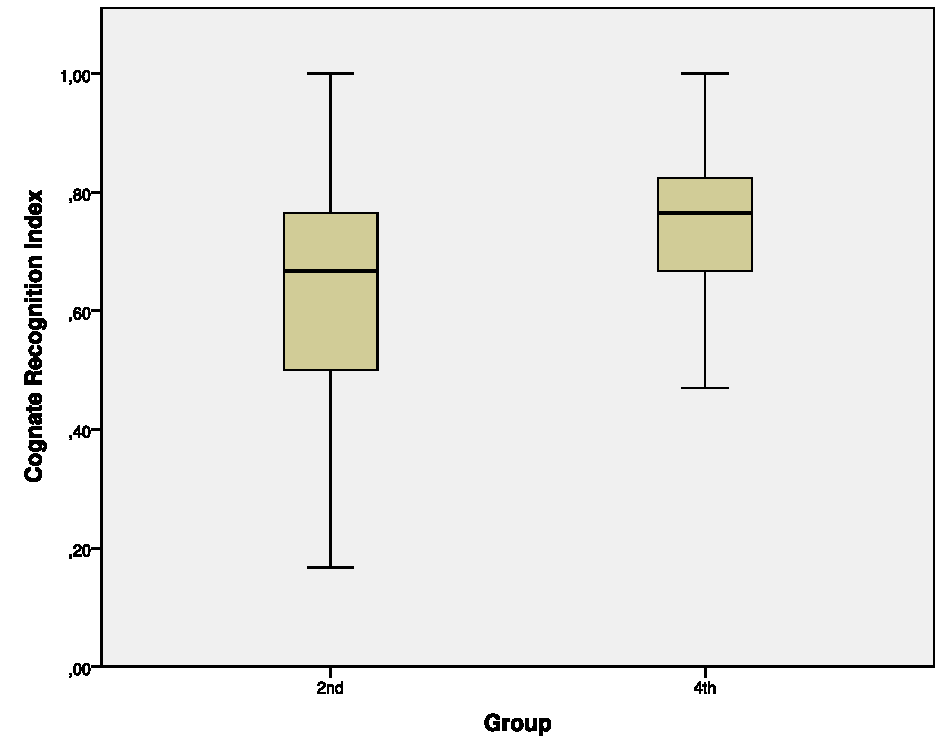
\includegraphics[width=.75\textwidth]{figures/CRI.pdf}%
\caption{\label{fig:munoz:1}Boxplot of CRI per age/grade level}
\end{figure}

\begin{figure}[p]
\caption{\label{fig:munoz:2}Boxplot of NCRI per age/grade level}
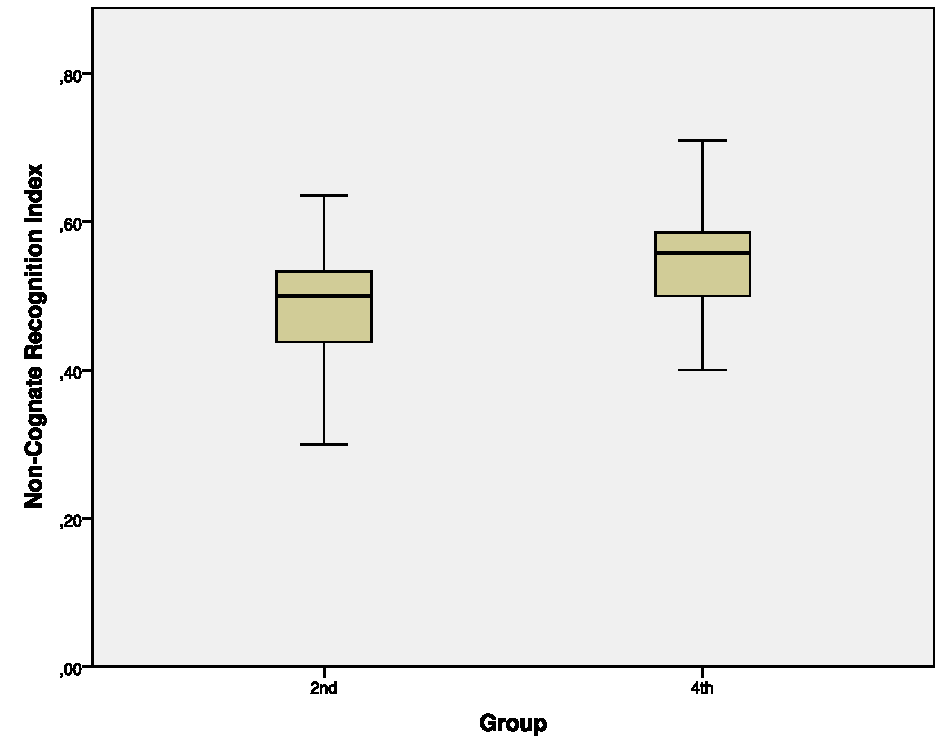
\includegraphics[width=.75\textwidth]{figures/NCRI.pdf}%
\end{figure}

Furthermore, to see if the difference in cognate recognition between the two age groups is statistically significant, an independent samples Mann-Whitney U test was conducted. The difference in cognate recognition between 9-year-old learners ($\text{median} = 0.76$) and 7-year-old learners ($\text{median} = 0.67$) was shown to be significant, $U = 4901$, $p < 0.001$, $r = 0.32$.  Another Independent Samples Mann-Whitney U test also showed that 9-year-olds ($\text{median} = 0.56$) outperformed 7-year-olds ($\text{median} = 0.50$) in non-cognate recognition. $U = 5176$, $p < 0.001$, $r = 0.38$. The effect sizes were moderate.

The second research question was concerned with the respective role of age (7 vs. 9 years) and amount of contact hours on cognate word recognition. A generalised linear mixed model (GLMM) analysis was calculated with CRI as the dependent variable. Participants were nested into age groups and groups into schools. Age and contact hours (the sum of English instruction and CLIL hours) were the fixed factors; there was no multicollinearity between these two variables ($\text{VIF} < 3$). School was introduced as a random intercept. The results, displayed in \tabref{tab:munoz:2}, show that there was a significant effect of age ($p < 0.01$), with the younger group scoring lower than the older group by about 0.12 points when all other factors were held constant. In contrast, the factor contact hours did not show a significant effect.

\begin{table}
\caption{Parameter estimates from the model for CRI\label{tab:munoz:2}}
\begin{tabular}{l S[table-format=-1.2e1] S[table-format=-1.2e1] S[table-format=-1.2] S[table-format=1.3] S[table-format=-1.3] S[table-format=1.3] }
\lsptoprule
    & \multicolumn{5}{c}{Fixed effects}\\\cmidrule{2-7}
Parameters & {Estimate} & {SE} & $t$ & {$p$-value} & \multicolumn{2}{c}{[95\% CI]}\\
\midrule
Intercept                                                & 0.77 & 0.08 & 10.13 & 0.000 & 0.620 & 0.921\\
Age/Grade\footnote{Age 7/Grade 2 is the reference group} & -0.12 & 0.04 & -2.91 & 0.004 & -0.199 & 0.038\\
Contact hours                                            &  6.24E-5 & 8.39E-5 & -0.74 & 0.458 & 0.000 & 0.000\\
\lspbottomrule
\end{tabular}
\end{table}

A similar analysis was conducted to assess the role of age and contact hours on these children’s recognition of non-cognate words. As displayed in \tabref{tab:munoz:3}, age was not a significant predictor of non-cognate word recognition, but there was a main effect of total hours of contact ($p < 0.01$). In other words, the higher the amount of contact hours with English, the more non-cognate words were known (although the increase that an average child would experience for every 1 extra hour is extremely small).

\begin{table}
\caption{Parameter Estimates from the Model for NCRI}
\label{tab:munoz:3}
\begin{tabular}{l S[table-format=1.3e1] S[table-format=1.3e1] S[table-format=-2.2] S[table-format=1.3] S[table-format=-1.3e1] S[table-format=1.3] }
\lsptoprule
 & \multicolumn{5}{c}{Fixed effects}\\\cmidrule{2-7}
Parameters & {Estimate} & {SE} & {\itshape t} & {$p$-value} & \multicolumn{2}{c}{[95\% CI]}\\
\midrule
Intercept                                                & 0.47     & 0.03      & 15.45 & 0.000 & 0.407    & 0.527\\
Age/Grade\footnote{Age 7/Grade 2 is the reference group} & -0.02    & 0.02      & -0.87 & 0.386 & -0.053   & 0.021\\
Contact hours                                            & 9.701E-5 & 3.578E-5 & 2.71  & 0.007 & 2.637E-5 & 0.000\\
\lspbottomrule
\end{tabular}
\end{table}

\section{Discussion}

In order to answer the first research question, which asked whether young Span\-ish-Catalan learners of English as a third language recognise cognate words better than non-cognate words, the proportion of correct answers to cognates and the proportion of correct answers to non-cognates were compared. The results indicated that these learners spontaneously relied on phonological similarity as a strategy to match the word they heard with the meaning provided by the picture they chose. As seen above, this cognate advantage was not found in the studies by \citet{UmbelEtAl1992} and \citet{UmbelOller1994} with Spanish-speaking children in English immersion programmes in the US. One possible explanation may be that they included all linguistic cognates in the analysis, some of which may not have been recognised by the children because of pronunciation differences. The results of the current study line up with most previous results, such as those by \citet{CunninghamGraham2000} also using the PPVT with English-monolingual and English-Spanish bilingual children and showing higher recognition of cognate words by the latter. A cognate advantage was also found in the study by \citet{KelleyKohnert2012} with Spanish-speaking English-language learners using the PPVT and a scale indexing cognate overlap and degree of difficulty. With young foreign language learners, \citet{GoriotEtAl2018} found that phonological similarity between Dutch and English words was a positive and significant predictor of pupils’ performance on the PPVT.

{Another finding of the current study is that, although both 7-year olds and 9 year-olds showed a large and significant difference in the proportion of correct answers to cognate items and non-cognate items, the older children significantly outperformed the younger children in both groups of items. This result is in line with the result obtained by \citet{MalabongaEtAl2008}, who found that the recognition of cognates by bilingual Spanish-English children increased with age in their first, third, and fifth graders. However, the test in that study was administered in written form, which may also explain the better performance of older children with higher levels of orthography and literacy. The current study also revealed a better performance by the older children group, but the test was administered in oral form, which avoids the confounding effect of literacy. The older advantage in cognate recognition has also been found in recent studies with bilingual children \citep{BosmaEtAl2019} and young foreign language learners (\citealt{GoriotEtAl2018}; \citealt{MuñozEtAl2018}). The explanation of this age advantage may be found in the concurrent development of metalinguistic skills (\citealt{Muñoz2006,Muñoz2014,KelleyKohnert2012}) and of L1 vocabulary size \citep{UnsworthEtAl2015} with age.}

{The issue of whether the older children’s advantage is an effect of age solely, or of previous amount of exposure to English as well, was addressed by the analyses pertaining to the second research question. A GLMM allowed us to account for the variability introduced by the different schools. The analyses showed that age was a very strong predictor of cognate recognition. On the other hand, the factor contact hours (including English instruction hours as well as CLIL hours) was not. This result is in line with the results of the first research question showing the significant effect of age on cognate recognition and confirms findings from previous research with bilingual children and with young foreign language learners (see above). The fact that the age gap was relatively small (2 years) also suggests that cognate awareness undergoes significant development between the two age points examined in the current study (age 7 and 9). The fact that age and contact hours could be dissociated here to some extent, because of the variability in the provision of English in the different schools, yields evidence that the effect of age on cognate-word recognition is stronger than the effect of contact hours in the learners in the current study. In contrast to the results relative to cognate word recognition, the results concerning non-cognate word recognition showed that hours of contact with English was a stronger explanatory factor of these children’s performance on non-cognate words than age. This finding was not unexpected and may be certainly attributed to the differences in proficiency and vocabulary size resulting from the different amounts of instruction and contact hours. However, the finding is valuable in showing a marked contrast between the results from cognate recognition and from non-cognate recognition, respectively, validating and highlighting the strong influence of age and cognate awareness on the former.}

\section{Conclusion and future perspectives}

This study examined young learners’ recognition of English-Spanish/Catalan cognate words through the analysis of their performance on the PPVT. It provided evidence of a cognate advantage in two different age groups (age 7 and 9) as well as evidence of an age advantage in that the older group outperformed the younger group in cognate recognition. The strong influence of age as an indicator of children’s stage of cognate awareness has been highlighted by the results that have contrasted the effects of age and contact hours on cognate and non-cognate word recognition.

 {Based on these findings, several pedagogical implications can be inferred. The study has revealed a cognate effect in young foreign language learners who have not been instructed to rely on cross-linguistic similarities. Teachers could use this incipient cognate awareness and foster it in the classroom to help young learners build a substantial L2 vocabulary that acts as a springboard for further L2 development, which would maximise classroom English language learning. Later on, teachers could capitalise on learners’ spontaneous recognition of phonological cognates to guide them through the phonological rules in the two languages (and the respective grapho-phonemic rules to enhance their recognition of written words; \citealt{LázaroIbarrola2010}) in order to improve their vocabulary and comprehension.}

 {This study is not without limitations. The first one is the use of the PPVT itself. Although the PPVT is probably the most popular test in this area, it may not be totally adequate for bilingual or foreign language learners because it was normed on a monolingual population. In addition, a test especially designed to measure awareness of cognate pairs between specific languages may be preferable (see \citealt{GoriotEtAl2018,LesniewskaEtAl2018}). Future research could look at larger age differences to better appreciate changes in cognate recognition with age. Longitudinal studies could also inform us of the developmental course. The design of future studies could also try to control for the variable amount of contact with the target language in order to shed more light on the respective predictive power of the two variables in different combinations of age and amount of contact hours (including out-of-school hours; see \citealt{MuñozEtAl2018}).  Finally, an issue that remains to be explored is the relationship between the cognate effect and proficiency levels that are higher than the beginner levels in this study, since there is some evidence of a decrease in cognate effect with adult foreign language learners with intermediate proficiency levels (i.e., at B1 in \citealt{CasaponsaEtAl2015}). Such a study should likely be conducted with older children than those in the current study, who will be expected to have reached higher proficiency levels.}


\section*{Acknowledgments}

This study was funded by the grant SGR 560 awarded to the GRAL group by AGAUR. I am very grateful to the schools and children that participated in the study, and to Ferran Gesa, Geòrgia Pujadas, and Radha Chandy for their help with the data.


\appendixsection{List of Spanish/Catalan Cognates in the PPVT (Sets 1--11)}

\begin{multicols}{2}\noindent
banana  – \textit{banana/banana} \\
bus  – \textit{(auto)bús/(auto)bús}\\
painting  – \textit{pintando/pintant}\\
dancing  – \textit{danzando/dansant}\\
lamp  – \textit{lámpara/làmpada}\\
castle  – \textit{castillo/castell}\\
penguin  – \textit{pingüino/pingüí}\\
fountain  – \textit{fuente/font}\\
tunnel  – \textit{túnel/túnel} \\
diamond  – \textit{diamante/diamant} \\
calendar  – \textit{calendario/calendari} \\
panda  – \textit{panda/panda}\\
cactus  – \textit{cactus/cactus}\\
dentist  – \textit{dentista/dentista} \\
floating  – \textit{flotando/flotant} \\
uniform  – \textit{uniforme/uniforme} \\
gigantic – \textit{gigantesco/gegantí\,(gegantesc)}\\
violin  – \textit{violin/violí} \\
group  – \textit{grupo/grup} \\
globe  – \textit{globo/globus} \\
chef  – \textit{chef/xef} \\
flamingo  – \textit{flamenco/flamenc} \\
chimney  – \textit{chimenea/xemeneia} \\
vegetable  – \textit{vegetal/vegetal} \\
hyena  – \textit{hiena/hiena} \\
horrified  – \textit{horrorizado/horroritzat} \\
pigeon  – \textit{pichón} \textit{(paloma)/colom} \\
flaming  – \textit{flambeado/flamejat}\\
aquarium  – \textit{acuario/aquari} \\
reptile  – \textit{reptil/rèptil}\\
canoe  – \textit{canoa/canoa} \\
directing  – \textit{dirigiendo/dirigint} \\
digital  – \textit{digital/digital} \\
dissecting  – \textit{diseccionando/diseccionant}\\
predatory  – \textit{predatorio/predatori} \\
hydrant  – \textit{hidrante/hidrant} \\
surprised  – \textit{sorprendido/sorprès}\\
palm   – \textit{palma/palma} \\
clarinet  – \textit{clarinete/clarinet} \\
kiwi  – \textit{kiwi/kiwi} \\
interviewing\,–\,\textit{entrevistando/entrevistant} \\
pastry – \textit{pastel/pastís}\\
assisting  – \textit{asistiendo/assistint}  \\
fragile  – \textit{frágil/fràgil} \\
solo  – \textit{solo/sol} \\
inflated  – \textit{inflado/inflat} \\
trumpet  – \textit{trompeta/trompeta} \\
rodent  – \textit{roedor/rosegador}
\end{multicols}

{\sloppy\printbibliography[heading=subbibliography,notkeyword=this]}
\end{document}
